\chapter{Implementierung der Webadministration}
\label{cha:impl_web}

Die Web Administration stellt die zentrale Kontrolleinheit des gesamten Projekts dar. Über die Web Administration werden sämtliche Einträge der Datenbank verwaltet, dies schließt neben der Benutzer- und Geräteverwaltung ebenfalls die Verwaltung aller Regale und Produkte ein.


\section{Technologische Grundlagen}

Die Administrationsoberfläche ist als Webapplikation und im Speziellen als Single-Page-Applikation konzipiert, d.h. sie besteht grundlegend aus einer einzigen Webseite, deren Layout (wie für Webseiten üblich) auf \ac{HTML} und \ac{CSS} aufgebaut ist. Die einzelnen Ansichten (Views) der Anwendung sowie jegliche dynamische Interaktionsprozesse werden über \acl{JS} als clientseitige Scriptsprache gesteuert. Dabei werden auch Daten oder Views im Hintergrund asnychron über \ac{AJAX} nachgeladen. Durch dieses Grundkonzept werden viele Ladevorgänge der kompletten Webseite vermieden und nur die Daten nachgeladen, die im Einzelnen benötigt werden -- dies sorgt für eine bessere Performance der Anwendung und somit eine bessere User Experience.\\

Das Layout selbst ist \emph{responsive}, d.h. es passt sich flexibel an die gegebene Bildschirmgröße des Ausgabegerätes durch eine optimiertes Layout (veränderte Anordnung von Seitenelementen, optimierte Platznutzung) an. Dadurch ist die Webadministration nicht nur für die Nutzung am Desktop-PC und großen Bildschirmen, sondern auch für die Verwendung auf Tablets und Smartphones gerüstet, sollte die Webanwendung im gesamten Netzwerk verfügbar sein (siehe Architektur).\\

Wie bereits in der Architektur angedeutet, läuft die Webadministration serverseitig mit der Scriptsprache \ac{PHP}. Hierüber werden Inhalte und Layoutkomponenten vorgeneriert und abhängig von den Parametern der clientseitigen Anfragen ausgeliefert. Auch die Validierung von Formularanfragen, sowie die Verbindung zur Datenbank und Datenbank-Abfragen werden über \ac{PHP} durchgeführt. Für die Datenbank selbst wird wegen der guten Kompatibilität mit PHP auf MySQL gesetzt.\\

Unter bestimmten Bedingungen (z.B. Sicherheitsvorschriften oder technische Einschränkungen) könnte die Ausführung von JavaScript im Browser des Anwenders nicht möglich sein. Die Webadministration ist in ihrer Funktionalität zu einem großen Teil auch ohne aktiviertes \acs{JS} lauffähig, indem die statischen Fallback-Links und Standardfunktionalitäten greifen, die via JavaScript sonst geblockt und eigene Interaktionsmethoden ersetzt werden. Dennoch lassen sich Teile der Anwendung ohne Einsatz von JavaScript nur sehr aufwändig umsetzen; als Beispiel dafür sei hier der Shelf Designer genannt, der im Folgenden noch näher beschrieben wird und ohne \acs{JS} nicht funktionsfähig ist.\


\section{Bereiche und Funktionen}

Das Layout der Webadministration ist in eine Navigationsleiste, eine Subnavigation und einen Inhaltsbereich aufgeteilt. Über die Navigationsleiste können die funktionalen Hauptbereiche geöffnet werden, die jeweils in der Subnavigation noch über Unterseiten verfügen. Der Inhaltsbereich enthält häufig Tabellen, die rechts eine Spalte mit Buttons für Aktionen zu einem Eintrag der Tabelle bereit halten. Tabellen, die wegen einer hohen Anzahl an Einträgen sehr lang werden würden, werden dabei automatisch auf mehrere Seiten verteilt, die über eine dann eingeblendete Seitennavigation geöffnet werden können. Die restlichen Views sind i.d.R. Formulare (z.B. für \emph{Neue Produkt anlegen} oder, bereits vorausgefüllt, \emph{Produkt bearbeiten}).\\

In den folgenden Kapiteln sollen die Bereiche der Webadministration ausführlich vorgestellt werden. Auf eine detaillierte Aufführung der betroffenen Daten und Felder wird dabei zwecks Übersichtlichkeit verzichtet -- diese wurden bereits in der Datenbank-Architektur (Kapitel \ref{sec:architektur_datenbank}) genauer erläutert.


\subsection{Produkte \& Einheiten}

\begin{figure}[H]
	\centering
	{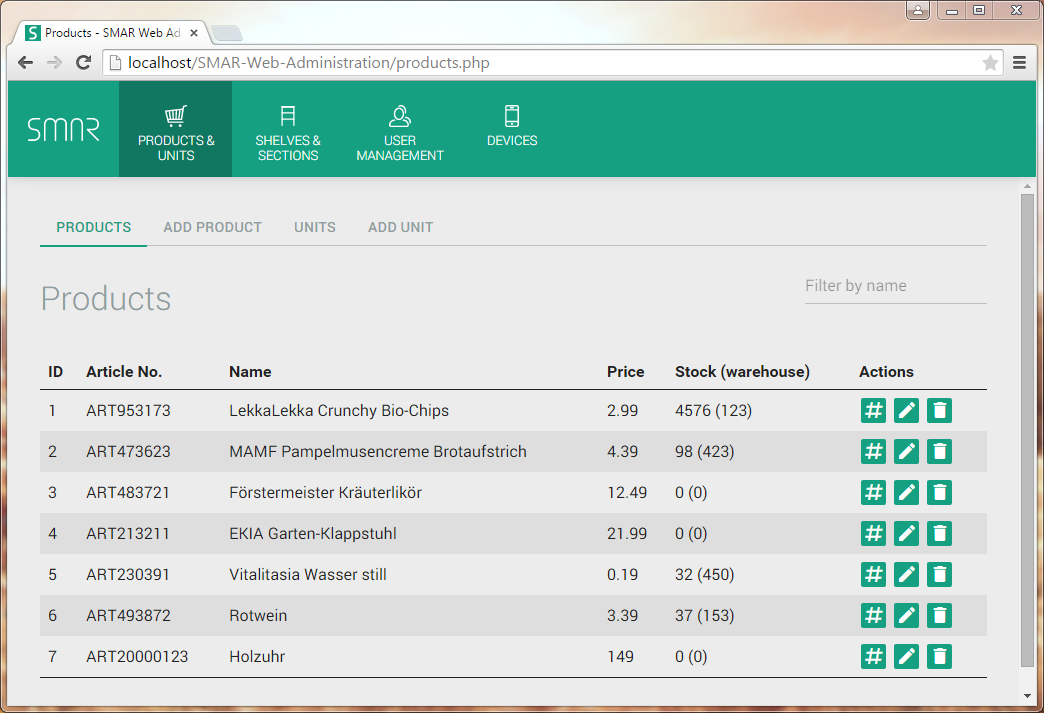
\includegraphics[width=\textwidth]{Bilder/Abbildungen/webadmin_products.png}}
	\caption{Produktübersicht in der Webadministration (Screenshot)}
	\label{fig:webadmin_products}
\end{figure}

In diesem Bereich der Webadministration können alle wesentlichen Aspekte rund um Produkte und die Einheiten, in denen Produkte auftreten können, verwaltet werden.\\

Als erstes wird eine Produktübersicht in Listenform angezeigt, über welche alle vorhandenen Produkte gefunden werden können. Zu einem Produkt werden die wesentlichen Informationen angezeigt, um ein Produkt identifizieren zu können, sowie der aktuelle Warenbestand eines Produktes. Über die Aktionen kann ein Produkt bearbeitet oder gelöscht werden, sowie die entsprechenden Produkt-Einheiten-Mappings angezeigt werden, die im Folgenden noch erläutert werden.\\

Auf einer Unterseite, erreichbar über die Subnavigation, kann über ein Formular ein neues Produkt angelegt werden, indem die notwendigen Informationen angegeben werden. Die notwendigen Abhängigkeiten zu anderen Tabellen werden dabei von der Webadministration automatisch angelegt. Analog gibt es ein Formular zum Anlegen von Einheiten für Produkte.\\

Zur Anzeige der vorhandenen Produkteinheiten gibt es eine Einheitenliste in einem eigenen View. Dieser gleicht (bis auf die dargestellten Informationen zu Einheiten) genau der Produktübersicht. In der Einheitenübersicht können ebenso einzelne Einträge betrachtet, bearbeitet und gelöscht werden; außerdem können auch hier für einzelne Einheiten die entsprechenden Produkt-Einheiten-Mappings angezeigt werden.\\

Ein nicht über die Subnavigation zugänglicher View sind die Produkt-Einheiten-Mappings. Diese Ansicht öffnet sich, wenn sie über die Produkt- oder Einheitenliste ausgewählt wird, und zeigt auf, welche Einheiten einem Produkt zugeordnet sind. In diesem View können die Zuordnungen auch bearbeitet, sowie neue Zuordnungen hinzugefügt werden. Die Produkt-Einheiten-Mappings sind z.B. wichtig zur Erkennung von Kartons, die eine größere Menge eines Produktes enthalten. Für diesen Zweck kann ein eigener Barcode pro Produkt-Einheit-Mapping gespeichert werden.


\subsection{Regale \& Fächer}

In diesem Bereich der Webadministration können die Regale auf der Verkaufsfläche sowie in dem Zusammenhang auch zugehörige Regalfächer angelegt und bearbeitet werden.\\

Wie auch bei Produkten und Einheiten gibt es eine Unterseite mit einer Auflistung aller vorhandenen Regale. Die Funktionen sind grundsätzlich die selben wie bei der Produktliste: einzelne Einträge der Tabelle können bearbeitet oder gelöscht werden. Zusätzlich gibt es bei Regalen die Aktion, den Shelf Designer zu öffnen.\\


\subsection{Shelf Designer}

\begin{figure}[H]
	\centering
	{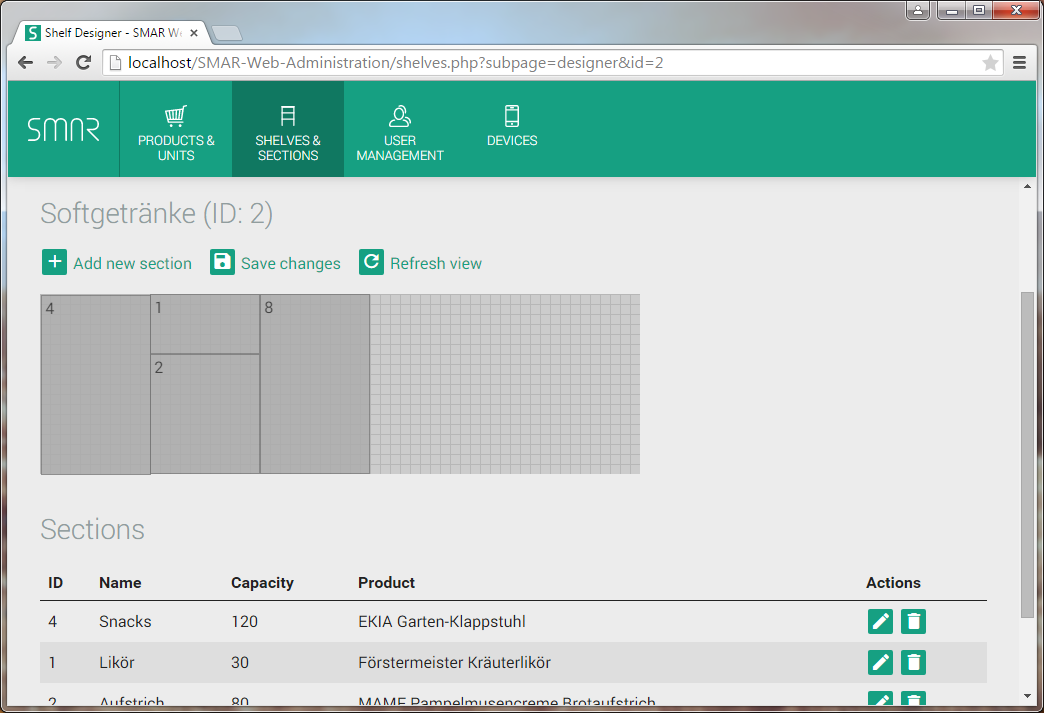
\includegraphics[width=\textwidth]{Bilder/Abbildungen/webadmin_shelves_designer.png}}
	\caption{Shelf Designer in der Webadministration (Screenshot)}
	\label{fig:webadmin_shelves_designer}
\end{figure}

Der Shelf Designer ist ein Tool in der \acs{SMAR} Webadministration, mit dessen Hilfe die Fächer eines Regals einfach angeordnet werden können. Wie in Abbildung \ref{fig:webadmin_shelves_designer} ersichtlich, besteht der Shelf Designer aus einer Arbeitsfläche, welche die Größe des zu bearbeitenden Regals hat. Auf der Arbeitsfläche sind die Regalfächer entsprechend ihrer in der Datenbank hinterlegten Position und Größe angeordnet.\\

Die Anordnung der Regalfächer kann per Drag \& Drop direkt verändert werden. Ebenso ist die Größenänderung durch Ziehen am Rahmen oder an den Ecken eines Fachs möglich. Auf dem Regal liegt dabei ein Grundraster mit einem Linienabstand von 10 Pixeln, wobei diese 10cm in Bezug auf die realen Maße des Regals entsprechen. Wird ein Regalfach bewegt oder in seiner Größe verändert, so ist dies nur entlang dieses Grundrasters möglich, alle Bewegungen rasten an den Grundlinien ein. Dadurch wird der Gestaltungsprozess für den Anwender deutlich vereinfacht. Um die Änderungen an der Regalanordnung letztendlich zu speichern, muss dieser nur auf Speichern drücken (\emph{Save changes}).\\

Neue Regalfächer lassen sich hier über einen Button anlegen. Im Gegensatz zu anderen Bereichen der Webadministration öffnet sich das Formular für eine neue  Section in einem Overlay, um den Arbeitsfluss mit dem Shelf Designer nicht zu unterbrechen. Im Formular muss zwingend ein verknüpftes Produkt eingegeben werden, welches dem Regalfach zugeordnet wird -- es muss also vorher ein Produkt zur Auswahl existieren. Nach Anlegen der neuen Section wird der Shelf Designer automatisch aktualisiert und enthält bereits die neue Section. Unter der Arbeitsfläche befindet sich eine Tabelle aller enthaltenen Regalfächer mit den üblichen Aktionen zum Bearbeiten und Löschen.\\


\subsection{Rechteverwaltung}
\label{cha:rechteverwaltung_web}
Die Web Administration stellt die zentrale Kontrolleinheit des gesamten Projekts dar. Über die Web Administration werden sämtliche Einträge der Datenbank verwaltet, dies schließt neben der Benutzer- und Geräteverwaltung ebenfalls die Verwaltung aller Regale und Produkte ein.\\
Dies sollte selbstverständlich ausschließlich durch autorisierte Personen durchführbar sein.\\

Die folgenden Kapitel befassen sich mit der Identifikation (\acs{AuthN}) und mit der Berechtigungskontrolle (\acs{AuthZ}) eines Benutzers gegenüber dem Webserver.

\subsubsection{\acf{AuthN}}
Ruft ein Benutzer eine URL der Webadministration auf, so wird zunächst überprüft, ob bereits eine mit Inhalt gefüllte \ac{PHP}-Session besteht, ist dies nicht der Fall wird der Benutzer auf die Login-Seite weitergeleitet. Der Benutzer hat nicht die Möglichkeit ohne \acl{AuthN} auf die Startseite oder eine Unterseite der Anwendung zu gelangen. Dementsprechend können ebenfalls keine Funktionen aufgerufen werden.\\
Ein Zugriff auf die \ac{REST} \ac{API} ist ohne Anmeldung ebenfalls nicht möglich, da der \ac{JWT} erst bei der Anmeldung generiert wird und Anfragen ohne gültigen \ac{JWT} abgebrochen werden.\\

Die Login-Seite hält ein \ac{HTML}-Formular mit zwei Eingabe-Feldern bereit, die die Eingabe des Benutzernamens und des Passworts ermöglichen. Diese Daten werden durch Absenden des Formulars an ein \ac{PHP}-Skript auf dem Server verschickt. Dieses Skript ruft den Eintrag der Datenbank ab, bei dem der Benutzername mit dem eingegebenen Namen identisch ist. Dem eingegebenen Passwort wird anschließend der Salt-Wert, der dem Benutzer in der Datenbank zugeordnet ist, angehängt und das zusammengesetzte Passwort wird mit dem SHA256-Verfahren gehasht. Das Passwort in der Datenbank wurde ebenfalls mit dem selben Verfahren gehasht und sollte daher identisch mit dem gehashten eingegebenen Passwort sein. Hat die Anfrage nach dem Benutzernamen einen Eintrag zurückgeliefert und die gehashten Passwörter sind identisch, so war der Login erfolgreich.\\
Bei einem erfolgreichen Login werden anschließend folgende Daten in einer neu erstellten \ac{PHP}-Session gespeichert:
\begin{itemize}
	\item Benutzer-ID (Primary Key der Datenbank)
	\item Benutzername
	\item Vorname
	\item Nachname
	\item gehashtes Password
	\item Personalnummer
	\item Berechtigungsstufe
	\item Loginzeit (Datum + Uhrzeit)
	\item Zeit seit dem letzten Seitenaufruf (Datum + Uhrzeit)
	\item ein gültiger \ac{JWT} zur Authentifizierung gegenüber der \ac{REST} \ac{API}\footnote{Siehe Kapitel \ref{cha:jwt} \nameref{cha:jwt}}
\end{itemize}
Der \ac{JWT} wird im Rahmen der Session-Erstellung generiert.\\
Nach Generierung der Session wird nun die Startseite der Anwendung angezeigt.\\
Sollte der Login-Vorgang aufgrund einer ungültigen Benutzername/Passwort-Kombination so wird die Login-Seite mit einer entsprechenden Fehlermeldung erneut angezeigt.\\

Das Hash-Verfahren für das Passwort, so wie ein individueller Salt-Wert pro Benutzer stellen eine Authentifizierung nach aktuellem Standard mit hoher Sicherheit dar. Auch wenn einem Angreifer das Auslesen der Benutzerdaten aus der Datenbank gelingt, kann er das Passwort eines Benutzers und somit den Zugriff mit einer vorgefertigten Rainbowtabelle nicht erlangen. Er muss eine große, für jeden Benutzer individuelle Rainbowtabelle anlegen, die bei einer Passwortlänge von 6 bis 9 Zeichen (in \ac{SMAR} Länger!) bei mindestens 62 möglichen Zeichen (A-Z,a-z und 0-9) plus 64 Byte (Salt-Wert-Länge) bereits bis zu 1000 Petabyte groß ist.\footnote{$\sum_{n=6}^{9} 62^{n}*(n+64)=1004$ Petabyte (keine Komprimierung)}\\

Werden nach einem erfolgreichen Login weitere Unterseiten aufgerufen oder Anfragen über direkte Links an den Server gestellt, so wird vor Ausführung des aufgerufenen Skripts ein anderes Skript eingefügt und ausgeführt, dass die Session kontrolliert. Dazu wird zunächst überprüft, ob eine Session mit Inhalt existiert. Ist dies nicht der Fall wird man, wie oben beschrieben, auf die Login-Seite weitergeleitet. Ist die Session aktiv werden zunächst die in der Session gespeicherten Daten (wie \zB der Benutzername) mit der Datenbank abgeglichen. Dadurch wird sichergestellt, dass es sich um eine gültige Session handelt und der Benutzer in der Datenbank existiert. Anschließend wird die Session auf einen möglichen Timeout untersucht. Dazu wird die aktuelle Zeit mit der letzten Aktivität und der Loginzeit, die beide in den Session-Daten abgespeichert sind, verglichen. Ein Timeout liegt vor, wenn:
\begin{itemize}
	\item Die letzte Aktivität (also der letzte Mausklick auf der Administrationsoberfläche) länger 12 Minuten her ist.
	\item Der Benutzer bereits länger als 24 Stunden angemeldet ist.
\end{itemize}
Bei einem Timeout wird der Benutzer ebenfalls zurück auf die Login-Seite, mit einer Timeout-Fehlermeldung, weitergeleitet. Dies stellt sicher, dass ein unbefugter Benutzer keinen Zugriff aufgrund eines für längere Zeit unbeaufsichtigten Computers bekommt. Außerdem wird sichergestellt, dass ein Benutzer nicht über mehrere Monate angemeldet bleiben kann und somit womöglich Rechte behält, die er laut Datenbank nicht mehr besitzt. Die Rechte werden, um die Performanz gewährleisten zu können, nicht bei jedem Aufruf mit der Datenbank abgeglichen.\\
Dieses Skript zur Session-Überprüfung wird auf jeder Unterseite - zusammen mit der Konfigurationsdatei - neu geladen und ausgeführt. Ein unberechtigter Benutzer hat somit keine Möglichkeit eine Aktion - auch nicht über direkte Links - ohne \acl{AuthN} auszuführen.\\

Die \ac{REST} \ac{API} verhält sich dem Skript zur Session-Überprüfung ähnlich. Bevor eine Anfrage von \ac{REST} bearbeitet wird, wird eine Funktion ausgeführt, die den \ac{JWT} auf Gültigkeit überprüft. Dieser wird dazu zunächst dekodiert\footnote{Siehe Kapitel \ref{cha:jwt} \nameref{cha:jwt}} und anschließend werden die im Token gespeicherten Daten mit der Datenbank abgeglichen. Nur bei einem erfolgreichen Abgleich wird die Anfrage bearbeitet.

\subsubsection{\acf{AuthZ}}
Im Gegensatz zu den Benutzern der \ac{VR}-Geräte, die entweder durch ihre Aufgabe volle Berechtigung auf den \ac{AR}-Geräten oder keine Berechtigung benötigen und es somit keine verschiedene Berechtigungsstufen benötigt, gibt es in der Web Administration verschiedenste Benutzern mit unterschiedlichen Berechtigungen im Unternehmen.\\
Während der Filialleiter sowohl Zugriff auf die Benutzerverwaltung, als auch auf die Regal- und Produktverwaltung haben sollte, so sollte ein Mitarbeiter, der für die Warenannahme und -einräumung beauftragt wurde, keinen Zugriff auf die Benutzerverwaltung haben.\\
Vor Allem durch die Benutzerverwaltung ist hier ebenfalls auf rechtliche Bestimmungen zu achten. § 3a Satz 2 \acs{BDSG}\footnote{\acf{BDSG}}:
\begin{quote}
	\glqq \textit{Die Erhebung, Verarbeitung und Nutzung personenbezogener Daten und die Auswahl und Gestaltung von Datenverarbeitungssystemen sind an dem Ziel auszurichten, so wenig personenbezogene Daten wie möglich zu erheben, zu verarbeiten oder zu nutzen. Insbesondere sind personenbezogene Daten zu anonymisieren oder zu pseudonymisieren, soweit dies nach dem Verwendungszweck möglich ist und keinen im Verhältnis zu dem angestrebten Schutzzweck unverhältnismäßigen Aufwand erfordert.}\grqq
\end{quote}
sagt aus, dass auch die Nutzung von personenbezogenen Daten, wie sie in der Benutzerverwaltung abgespeichert werden müssen, so weit wie möglich reduziert werden soll. Ein Mitarbeiter, der nicht im Personalmanagement angestellt oder mit Aufgaben der Benutzerverwaltung beauftragt ist, sollte somit auch keinen Zugriff auf personenbezogene Daten haben. Im Zweifelsfall wäre dieser Benutzer eventuell sogar unberechtigt diese Daten einzusehen.\\

Die Autorisierung von Benutzern konnte in \ac{SMAR} dahingehend vereinfacht werden, dass davon ausgegangen wurde, dass die verschiedenen Berechtigungsstufen aufeinander aufbauend sind. Das heißt jemand in einer höheren Berechtigungsstufe hat immer die Berechtigungen der darunterliegenden Berechtigungsstufe und darauf aufbauende Rechte. Eine niedrigere Berechtigungsstufe hat somit niemals Rechte, die eine höhere Stufe nicht besitzt.\\

Aus den Aufgaben dieses Projektes und der Berücksichtigung eventueller Gesetzesvorgaben ließen sich die folgenden acht Berechtigungsstufen herleiten:
%\begin{enumerate}
%	\item[0]: keine Berechtigung
%	\item[10]: Products, Units, Shelves, Sections lesen; keine Schreibberechtigung
%	\item[20]: Schreibberechtigung für Products \& Units
%	\item[30]: Schreibberechtigung für Bestellungen
%	\item[40]: Schreibberechtigung für Products, Units, Shelves \& Sections
%	\item[50]: Lese- und Schreibberechtigung für Geräteverwaltung
%	\item[60]: Lese- und Schreibberechtigung für die Benutzerverwaltung
%	\item[70]: Vollständige Berechtigung
%\end{enumerate}
\begin{figure}[H]
	\centering
	{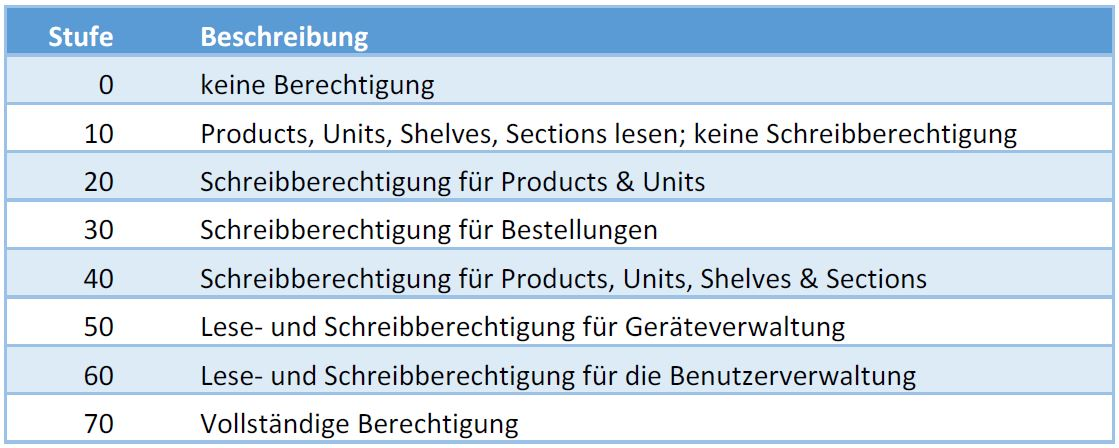
\includegraphics[scale=0.5]{Bilder/role_web.jpg}}
	\caption{Berechtigungsstufen in der Web-Administration}
	\label{fig:role_web}
\end{figure}
Wie im vorherigen Absatz beschrieben, besitzen höhere Berechtigungsstufen automatisch auch die Berechtigungen geringerer Stufen. Außerdem wurde darauf geachtet, dass späteres Erweitern der Funktionalität der Anwendung noch weitere Berechtigungsstufen erfordern könnten. Berechtigungsstufen wurden in Zehnerschritten durchnummeriert, einzelne Berechtigungsstufen können durch Nutzen der Einerschritte in vorhandene Stufen integriert werden ohne dass die Anwendung in bestehenden Programmteilen angepasst werden muss.\\

Berechtigungsstufe 0 gibt dem Benutzer keine Berechtigung die Anwendung zu benutzen, der Anmeldebildschirm wird nicht auf die Startseite weitergeleitet, sondern gibt eine Fehlermeldung \glqq Insufficient Permissions\grqq\footnote{zu Deutsch: \glqq mangelnde Berechtigung\grqq} zurück. Dies kann erforderlich sein, wenn einem Mitarbeiter gekündigt wurde, er aber aufgrund von \zB offenen Gehaltszahlungen noch nicht aus dem System gelöscht werden darf. Berechtigungsstufe 10 gibt Zugriff auf die Anwendung und auf die Basisfunktionalität, der Benutzer bekommt allerdings noch keine Schreibberechtigung. Dies ist für Mitarbeiter sinnvoll, die mit der Überwachung des Warenbestands beauftragt wurden, allerdings keine Berechtigung haben sollen, diesen zu verändern. Die darauffolgende Stufe 20 gibt dem Benutzer zusätzlich die Berechtigung auf die Produktverwaltung. Der Benutzer ist daher berechtigt Produkte zu verändern/hinzuzufügen oder zu löschen. Die Regalverwaltung ist hier noch nicht inbegriffen und wird erst in der Stufe 40 hinzugefügt. Dem Benutzer ist es nun erlaubt Regale, Regalstandorte und die Anordnung der Produkte innerhalb des Regales zu verändern. Darauffolgende Berechtigungsstufen 50, 60 und 70 dienen der Verwaltung und sind für die eigentliche Aufgabenerfüllung nicht mehr notwendig. Stufe 50 fügt die Berechtigung zur Geräteverwaltung hinzu, das heißt der Benutzer darf nun \ac{AR}-Geräte, wie \zB die Smartglass hinzufügen oder löschen. Stufe 60 fügt eine nach dem Gesetz sensible Berechtigung hinzu, nämlich den Lese- und Schreibzugriff auf personenbezogene Daten. Der Benutzer ist nun berechtigt andere Benutzer hinzuzufügen, zu löschen oder zu verändern (wie \zB Berechtigungen verändern). Das Ändern des Passworts des eigenen, angemeldeten Benutzers ist jedoch bereits ab Berechtigungsstufen größer als 0 verfügbar. Die letzte Stufe 70 gewährt volle Berechtigungen auf alle Komponenten der Web-Administration. Dies ist für Systemadministratoren und Filialleiter geeignet, in diesen Fällen muss ein ständiger Zugriff auf die gesamte Anwendung garantiert sein.\\

Die oben genannten Berechtigungsstufen werden in der Datenbank in der für die Benutzer zuständigen Tabelle (user\footnote{Siehe Kapitel \ref{sec:architektur_datenbank} \nameref{sec:architektur_datenbank}}) abgespeichert. Die Tabelle enthält die Spalte role\_web. In dieser Spalte wird für jeden Benutzer die entsprechende Berechtigungsstufe als zweistellige Nummer gespeichert. Greift der Benutzer nun auf die Anwendung zu, wird während der Anmeldung zunächst überprüft, ob die Berechtigung ungleich 0 (keine Berechtigung) ist und anschließend die Berechtigung in der Session gespeichert. Ruft man eine Komponente/eine Funktion innerhalb der Anwendung auf, so wird überprüft, ob die Berechtigungsstufe größer oder gleich (>=) der erforderlichen Nummer ist. Ist die Nummer größer oder gleich wird der Zugang gewährt und die Funktion aufgerufen, ansonsten wird die Anfrage mit der Fehlermeldung \glqq Insufficient Permissions\grqq\footnote{\glqq mangelnde Berechtigung\grqq} abgebrochen.

\subsubsection{Benutzerverwaltung}
Die Benutzerverwaltung ist ein Teil der \ac{SMAR} Web Administration und beschäftigt sich mit dem Verwalten der Benutzer. Die Benutzerverwaltung ist somit ein essentieller Teil für die Rechteverwaltung der Smartglass und der Web Administration.\\

Die Benutzerverwaltung besteht aus drei Unterseiten:
\begin{itemize}
	\item Passwörter ändern
	\item Benutzer editieren
	\item Neuen Benutzer anlegen
\end{itemize}
Wie im Kapitel Autorisierung beschrieben, ist die Benutzerverwaltung mit Ausnahme der \glqq Passwort ändern\grqq -Funktion nur von Benutzern mit einer Berechtigungsstufe von mindestens 60 zugänglich. Benutzer mit einer geringeren Berechtigungsstufe können ausschließlich ihre eigenen Passwörter ändern.\\

Auf dieser Seite können zwei Passwörter verwaltet werden. Das Passwort für die Web Administration und das Passwort für die Smartglass, welches in Form eines QR-Codes dargestellt wird.\\

Ändert ein Benutzer das Passwort für die Web Administration, wird durch die Anwendung zuerst ein neuer Salt generiert, dieser setzt sich aus folgenden drei Abschnitten zusammen:
\begin{itemize}
	\item einem Teil des Benutzernamens
	\item der aktuellen Zeit in ms (Beginn ab 01.01.1970 00:00 Uhr)
	\item einem Teil des Nachnamens
\end{itemize}
Dem neuen Passwort wird der mit dem SHA256-Verfahren gehashte Salt angehängt und das Passwort wird anschließend ebenfalls gehasht und in der Datenbank abgelegt.\\
Möchte ein Benutzer den Zugang zu der Brille ändern oder wiederherstellen hat er er die Möglichkeit sich einen neuen QR-Code generieren lassen, den aktuell gültigen QR-Code ausdrucken oder einen eigenen QR-Code zu aktivieren. Der neue Code, der wieder mit dem SHA256-Verfahren gehasht wird und somit aus 64 Zeichen besteht, wird durch die Anwendung aus folgenden Daten des Benutzers zusammengesetzt:
\begin{itemize}
	\item Aktueller Zeit
	\item Aufgeteiltem Salt des Benutzers
	\item Benutzername
	\item Einer Zufallszahl zwischen 0 und $2^{32}$ (32 Bit System) \bzw $2^{64}$ (64 Bit System)\footnote{{\citep{mt_rand}}}
\end{itemize}
Dieser Code \bzw der durch den Benutzer eingegebene String wird in der Datenbank gespeichert. Anschließend wird auf eine freie PHP-Library namens \glqq phpqrcode\grqq , die auf \url{http://phpqrcode.sourceforge.net/} veröffentlicht ist, zurückgegriffen. Diese interpretiert den String aus der Datenbank und wandelt ihn in einen QR-Code um. Die Library ist in \ac{SMAR} dabei so konfiguriert, dass sie den QR-Code sowohl als png und jpg-Datei zurückgibt und eine für die Kamera der Smartglass akzeptable Größe, Qualität und Genauigkeit hat.\\

Die anderen beiden Unterseiten bieten, für Benutzer mit einer Berechtigungsstufe größer als 60, das Editieren und Anlegen neuer Benutzer an. Im Gegensatz zu einer Standard Benutzerverwaltung werden hier jedoch keine E-Mail-Adressen, sondern Firmen interne Daten, wie \zB die Personalnummern und vor Allem die Berechtigungsstufen abgefragt. Darüber hinaus ist sie Benutzerverwaltungen, die man von bekannten \ac{CMS} und Web Administrationen kennt, ähnlich.

\subsection{Weitere Funktionen}

Die für diese Arbeit vorliegende Version der \acs{SMAR} Webadministration enthält nur die notwendige Funktionalität, um die Grundfunktionen der App auf der Smartglass bedienen zu können. Das Datenbankschema ist jedoch schon für weitere Funktionen ausgelegt, die das Shelf Management mit \acs{SMAR} noch besser unterstützen und erweitern. Diese sollen im Folgenden kurz angeschnitten werden.

\subsubsection{Bestellungsmanagement}
Die Warenannahme bei neuen Produktlieferungen dient nicht nur dazu, die Produkte im Lager für das System zu erfassen. Durch die Prozessierung der Warenannahme sollen auch vorausgegangene Bestellungen dahingehend überprüft werden, ob die gelieferte Ware der Bestellliste entspricht. Auch sollen Differenzen in diesem Schritt erfasst und anschließend an den Lieferanten weitergegeben werden, sodass dieser nachliefern bzw. -buchen kann.\\

Um diese Prozesse abbilden zu können, müssen Bestellungen im System vorliegen. Diese sollen über die Webadministration angelegt und verwaltet werden können, dabei können die Positionen der Bestellung direkt aus den Produkten und Einheiten des Systems zusammengestellt werden, wodurch auch bei der Warenannahme durch die Smartglass keine weiteren Mappings der Bestellliste auf das System notwendig wären. Da verschiedene Einzelhandelsketten unterschiedliche interne Bestellsysteme verwenden und diese wahrscheinlich nicht direkt mit dem \acs{SMAR}-System kompatibel sind, muss außerdem eine Schnittstelle bereitgestellt werden, über welche Bestelldaten zwischen den Systemen transferiert werden können. Ebenso muss eine Differenzliste bei Lieferabweichungen im notwendigen Format bereit gestellt werden.

\subsubsection{Market Map}
Eine weitere praktische Zusatzfunktion des Systems wäre eine Wegfindung bzw. Navigation über die Verkaufsfläche, die z.B. beim Einräumen mehrerer Produkte hilfreich sein könnte, um eine optimale Route von Regal zu Regal zu berechnen. Dafür ist Voraussetzung, dass die Beschaffenheit der Verkaufsfläche mit allen Regalen und ihren Positionen bekannt ist.\\

Für diesen Zweck soll die Filiale über die Webadministration als \emph{Market Map} angelegt werden können. Diese definiert die Maße der Verkaufsfläche sowie die Regalpositionen und -ausrichtungen. Dazu bietet sich eine Umsetzung ähnlich dem Shelf Designer als eingebettetes Tool an (Map Designer). Ist die Verkaufsfläche auf diese Weise definiert, kann diese mit geringem technischem Aufwand zur Wegfindung verwendet werden.

